\documentclass[a4paper]{article}
\usepackage{iwslt15,amssymb,amsmath,epsfig}
\usepackage{verbatim}
\usepackage{CJKutf8}
\usepackage{multirow}
\usepackage{newfloat}
\DeclareFloatingEnvironment[placement={!ht},name=Example]{mylist}
\newcommand{\ch}[1]{\begin{CJK}{UTF8}{gbsn}{#1}\end{CJK}}
\newcommand{\uch}[2]{\underbrace{\text{\ch{#1}}}_{\text{\ch{#2}}}}
\newcommand{\anony}[1]{\textit{[anonymized]}}
\setcounter{page}{1}
\sloppy		% better line breaks
%\ninept
%SM below a registered trademark definition
\def\reg{{\rm\ooalign{\hfil
     \raise.07ex\hbox{\scriptsize R}\hfil\crcr\mathhexbox20D}}}

%% \newcommand{\reg}{\textsuperscript{\textcircled{\textsc r}}}

\title{Integrating Encyclopedic Knowledge into Neural Network Language Models}

%%%%%%%%%%%%%%%%%%%%%%%%%%%%%%%%%%%%%%%%%%%%%%%%%%%%%%%%%%%%%%%%%%%%%%%%%%
%% Please make sure to keep technical paper submissions anonymous  !
%%%%%%%%%%%%%%%%%%%%%%%%%%%%%%%%%%%%%%%%%%%%%%%%%%%%%%%%%%%%%%%%%%%%%%%%%%
\name{Firstname Lastname}
%%%%%%%%%%%%%%%%%%%%%%%%%%%%%%%%%%%%%%%%%%%%%%%%%%%%%%%%%%%%%%%%%%%%%%%%%%
%% If multiple authors, uncomment and edit the lines shown below.       %%
%% Note that each line must be emphasized {\em } by itself.             %%
%% (by Stephen Martucci, author of spconf.sty).                         %%
%%%%%%%%%%%%%%%%%%%%%%%%%%%%%%%%%%%%%%%%%%%%%%%%%%%%%%%%%%%%%%%%%%%%%%%%%%
% \makeatletter
% \def\name#1{\gdef\@name{#1\\}}
% \makeatother
% \name{{\em Firstname1 Lastname1, Firstname2 Lastname2, Firstname3 Lastname3,}\\
%      {\em Firstname4 Lastname4}}
%%%%%%%%%%%%%%% End of required multiple authors changes %%%%%%%%%%%%%%%%%

%\address{Institute for Anthropomatics  \\
%Karlsruhe Institute of Technology, Germany \\
%{\small \tt firstname.lastname@iwslt.org}
%}
%
\begin{document}
\maketitle
%
\begin{abstract}
Neural models have recently shown big improvements in the performance of phrase-based machine translation. Recurrent language models, in particular, were a great success due to their ability to model arbitrary long context. In this work, we want to integrate global semantic information extracted from large independent knowledge bases into neural network language models. We propose two approaches for doing this: word class extraction from Wikipedia and sentence level topic modeling. 
The new resulting models exhibit great potential in counteracting data sparsity problems with additional independent knowledge. This approach of integrating global context information is not restricted to language modeling but can also be easily applied to any model that profits from context or further data resources, e.g. neural machine translation. Using this model has improved rescoring quality of a state-of-the-art phrase-based translation system by ... BLEU points.  We performed experiments on two language pairs.



\end{abstract}


%
\section{Introduction}
Recurrent neural network language models have recently shown great improvement in statistical machine translation, both during decoding and rescoring. The use of continuous word representations has achieved better generalizations of the data which effectively lowered data sparseness problems. Furthermore, the recurrent connections are able to model long range dependencies. Yet, most of these models strictly depend on monolingual and parallel data, which is sometimes not available in huge amounts or only for different domains, especially for low-resource languages.
This has motivated neural network language models that take multiple parallel streams of data as input instead of just the single form of surface words. These so called factors can be used to add additional information, e.g. POS or automatic word clusters, which helps mainly with morphologically rich languages (e.g. Romanian, German). However, so far the additional feature only pertained to syntactic or local context knowledge around the current word. Especially for languages with low resources, it is essential to also facilitate the use of other knowledge sources, e.g. encyclopedia knowledge. It is a useful source especially for learning general concepts, even more after the emergence of the Internet has led to an explosion of textual data. These data sources give insights into a variety of human endeavors waiting to be computationally analyzed.
In this paper, we study the integration of large independent knowledge bases in the form of encyclopedia, e.g. Wikipedia, into RNN-based language models and propose two solutions. 
First, we use  the factored model to integrate Wikipedia categories as one of the factors. In order to understand large unstructured datasets great achievements have been attained in latent concept learning in the area of text mining. Techniques include categorization of documents using latent semantic analysis and probabilistic topic modeling. In our case, we used techniques like tfidf, LSA and LDA to compute a real-valued topic vector for each sentence that is fed into the network as additional input. 
General word class and global topic features are used in combination with local contexts provided by recurrent neural models to improve lexical selection. 


\section{Related Work}
Language models are a critical component of many application systems, e.g. ASR, MT and OCR. However, language models have always faced the problem of data sparseness. Factored Language Models \cite{bilmes2003factored} introduced the use of a bundle of factors associated with a word which outperformed previous n-gram models without expanding the training data. For factors morphs, stems, POS and word class obtained using the SRILM's n-gram-class tool were used. \cite{koehn2007factored} replaced the single feature stream of surface words with multiple factors and integrated it into phrase-based statistical machine translation systems by breaking down the translation model into several steps that pertain to the translation of single factors which are all taken into account when the target word is generated.
After recurrent neural network models became a success in language modeling \cite{mikolov2010recurrent}, a factored input layer was employed in a model by \cite{wu2012factored} which uses a structured output layer based on word classes that was able to handle vocabulary of arbitrary size.
Motivated by multi-task learning in NLP, \cite{niehuesusing} proposed a multi-factor recurrent neural network language model which jointly predicts different output factors by mapping the output of the LSTM-layer to as many softmax layers as there are output factors, thus creating multiple distributions at the output layer. In the rescoring of an n-best list, this model can be included as either one additional feature or several features depending on whether the output is treated as a joint probability or individual probabilities.
However, a dedicated continuous space vector offers more flexibility and possibility to store additional side information, especially for complex higher-level concepts, e.g. topic distributions. In \cite{mikolov2012context} a first approach to use an additional vector for higher-level concepts was proposed. In their work, a vector instead of a single factor is associated with each word. However, this vector depended only on the  earlier local context of the word, neglecting the influence of the future context on a word's meaning. 
In fact, often the meaning of a word cannot be just derived from its preceding words but by content words in the entire sentence or surrounding sentences. 
Topic models play a great role in text mining because they summarize concepts in large amounts of documents into fewer topics by capturing word co-occurence information. Essentially, topic models can be divided into vector space models, e.g. LSA \cite{deerwester1990indexing}, and probability models, e.g. LDA \cite{blei2003latent}. 
The successful usage of Wikipedia to devise methods for computing semantic relatedness of documents was reported in \cite{gabrilovich2007computing} and \cite{strube2006wikirelate}.
Generative probabilistic models were employed in \cite{han2012entity} to link named entities in text documents by using information extracted from Wikipedia. 
In \cite{cucerzan2007large},\cite{bunescu2006using} vector space models are employed to resolve word disambiguations based on entities derived from Wikipedia.
Similar approaches were applied on other knowledge sources, such as WordNet \cite{hearst1992automatic}.
However, to our knowledge, it is the first time to combine both encyclopedic knowledge and neural language models.

\section{Integration of Side Information}
We studied two approaches to integrate encyclopedic information into neural language models.
First, we extracted for each word a corresponding label from Wikipedia. For this, we exploited the existing hierarchical page structure of Wikipedia and use the category label of a page as a factor input into the previously described factored neural language model.
Second, for each sentence a ranking of similar encyclopedia documents is calculated using vector space models, such as tfidf or LSA, and topic models, such as LDA. Based on the same underlying models a feature vector of the most similar documents to the current sentence is computed which is fed into a neural language model as additional input. The second approach is not limited to Wikipedia, but can be applied to any encyclopedia. To show the efficiency of this method independent from the underlying knowledge source we have crawled a Chinese lexicon from zdic.net \footnote{http://www.zdic.net/} for which we will present the results later on. 


\subsection{Word Level Information} \label{sec:word-level}
The motivation behind using general word categories from Wikipedia in association with words is to strengthen the relatedness of words in sentences that are correct translations but have a low score due to the translation model.
\begin{align}
\text{``A journalist writes articles for a column''}
\end{align}
Both of the following hypotheses, as shown in Example \ref{ex:wiki-cat}, are possible translation candidates in decoding:
\begin{mylist}
\caption{Two hypothese tagged with Wikipedia categories}
\newcommand{\uchx}[3]{\underbrace{\substack{\text{\ch{#1}}\\\text{#2}}}_{\text{\ch{#3}}}}
\begin{enumerate}
\item $\uchx{一位}{one}{NR}$ $\uchx{记者}{journalist}{新闻 (=news)}$ $\uchx{给}{for}{P}$ $\uchx{柱子}{column}{建筑(=archit.)}$ $\uchx{写}{write}{VV}$ $\uchx{文章}{article}{作品}$
\item $\uchx{一位}{one}{NR}$ $\uchx{记者}{journalist}{新闻 (=news)}$ $\uchx{给}{for}{P}$ $\uchx{专栏}{column}{新闻(=news)}$ $\uchx{写}{write}{VV}$ $\uchx{文章}{article}{作品}$
\end{enumerate}
\label{ex:wiki-cat}
\end{mylist}

 Even though the second translation is obviously the correct one, because ``column'' in the context of ``journalist'' and ``article'' refers to a newspaper section, the first translation is more likely according to the translation model since, generally, a column describes more often a pillar than a newspaper area. Since the main contextual word of ``column'', which is ``article'', is several words apart, translation tasks where the data does not originate from news or similar domains, or in case the data is so constrained in size that it has never seen the words ``column'' and ``journalist'' in the same context, the language model will fail to choose the correct translation.
Out approach solves this problem by tagging the nouns in the sentence with according Wikipedia categories. By doing so, the bond between column and journalist is reinforced by the their common factor \ch{新闻 (=news)} which contributes to a higher score for the correct translation. 



\subsubsection{Input representation}
A Wikipedia page, labeled with a title, is either an article or a category page which encompasses one or multiple pages.
We define the search space as the set of all page titles. Given a word, we search for the page with the same word as title and retrieve its category which is found at the bottom of the page.
%In case of multiple categories we pick the first one, which is usually the most general one.
In implementation, we downloaded the freely available Wikipedia dump to create a mapping of pages and their category offline. Using a threshold for the minimum number of elements in a categories, we pick recursively the parent of a category in case it does not meet the requirement, thus reducing the total number of associated articles which performed better in practice. In case no category is found at all, we resort to the default part-of-speech tag of a word.
One typical characteristic of Wikipedia is that most of its articles only refer to a small group lexical categories. For example, there are lots more articles about objects (nouns) than about activities (verbs). Fortunately, topic words are usually nouns, so it suffices to tag nouns for an improvement in model quality as suggested in  Example \ref{ex:wiki-cat}.

\subsubsection{Factored language model}
For training we used the factored language model proposed in \cite{niehuesusing}, which takes in one or multiple factors at the input layer and offers the option to factorize output layer. After concatenating the embeddings of the input factors into a single word embedding, this vector is send through one or multiple LSTM-based layers before projected onto the factored output probabilities. The instance of the model we used for our purposes, takes two factors, the surface form and the Wikipedia word category. These are mapped to an embedding vector of size 100, which is the same size as the first LSTM-layer. For the second LSTM-layer we used 200 nodes. We only used one factor for the output, the surface form of the next word.


\subsection{Sentence Level Information} \label{sec:sentence-level}
The idea to use a dedicated topic vector is motivated by a more flexible representation of information and methods that are capable of drawing correlations betweens words independent of their distance.
For example, the sentence 
\begin{align}
\text{``Columns contain articles written by journalists''}
\end{align}
exhibits several problems. First, when translated into a low-ressource languages, e.g. Romanian, some of the topic words do not have their own Wikipedia entries, so we cannot take full advantage of the first approach. Second, the contextual word of ``columns'', which is ``journalists'', appears later in the sentence, thus recurrent models only considering the earlier context will fail. 
This motivated to take words in the entire sentence, both left and right of the current word -  unlike \cite{mikolov2012context}, to create a topic vector by searching through Wikipedia contents to find topic-related articles, in the above example news related articles. By compressing the information of these articles into a vector which is associated with each word, we can improve the translation of single words by considering global topic information spanning neighboring words. 
To create a ranking of similar documents and their representation to a given sentence we employ vector space models, such as the tf-idf \cite{salton1986introduction} and latent semantic indexing model \cite{bradford2008empirical}, as well as probabilistic models, such as latent dirichlet allocation \cite{blei2003latent}. After representing the sentences and cleaned encyclopedia articles as bag-of-words, we query for each sentence the most similar documents from the total set of encyclopedia articles. These documents provide general information, such as higher-level concepts, about the current sentence. Based on the chosen model the best documents are transformed into vector representations and the averaged sum of the vectors is used as the additional feature input for the extended neural language model. This process is illustrated by Figure \ref{fig:flow}.
\begin{figure} 
\centering 
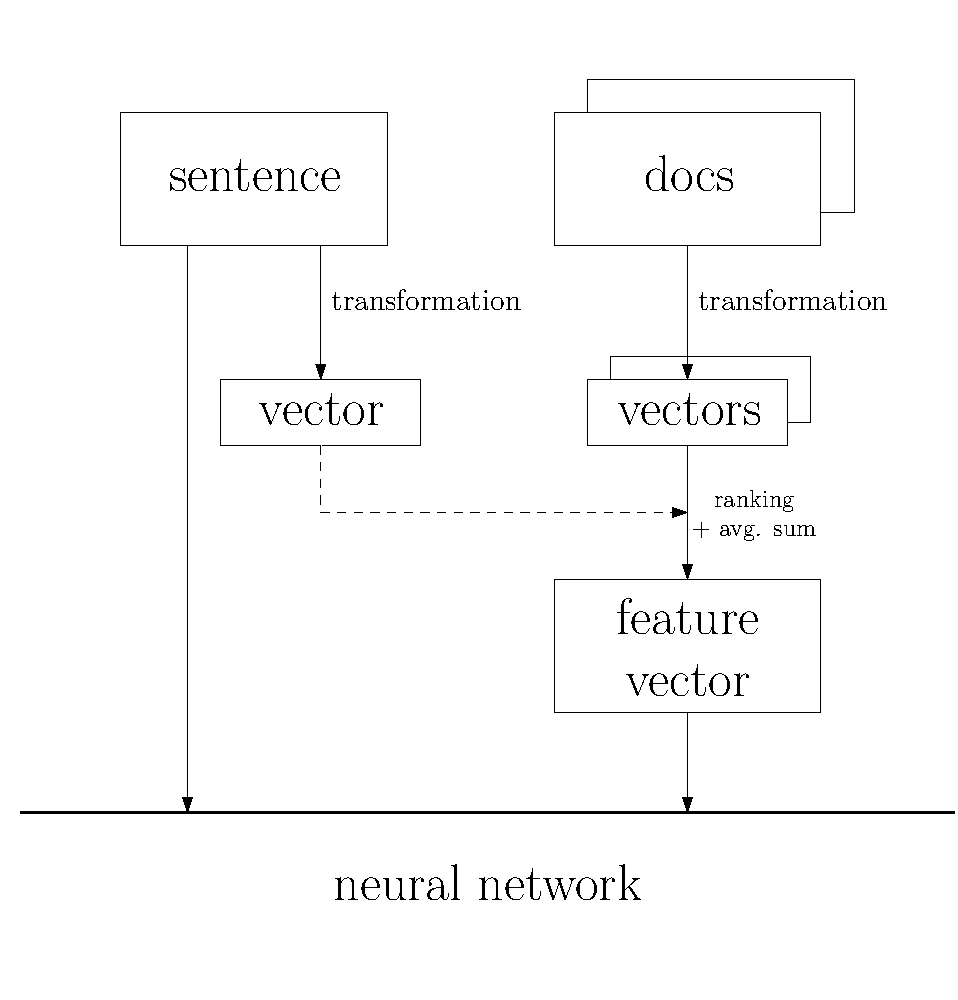
\includegraphics[width=\columnwidth]{flow.pdf}
\caption{Flow}
\label{fig:flow}
\end{figure}

\subsubsection{TF-IDF}
Tf-idf \cite{salton1986introduction} is a co-occurrence measure and determines the importance of a word to one or multiple documents. Having the capability of grading down term appearing in multiple documents, tf-idf is computed by multiplying a local component (term frequency or $tf$) with a global component (inverse document frequency or $idf$).
Using the cosine distance a ranking of similar documents for a given sentence query can be determined.
For a predefined number of top documents $n$ we determine the averaged tf-idf value of the best $n$ documents to a query, which we denote with $\text{top-doc-tfidf}(q, D, n)$.
This vector constitutes the sentence level semantic information which is fed into a RNNLM together with the surface data stream.
Shortcomings of this model include the inability to reduce the description length of the document, since words are only replaced with values. Also, it does not tell much about the statistical structure within and between documents.


\subsubsection{Latent Semantic Indexing}
Latent semantic analysis (LSA) \cite{deerwester1990indexing} is a method that discovers hidden concepts in documents by using single value decomposition (SVD) on the set of documents $D$.
LSA uses a term-document matrix $A$ with rows corresponding to terms and columns corresponding to documents. The entry $A_{i,j}$ equates to $tfidf(t_i, d_j, D)$. SVD decomposes $A$ into $U$, $\Sigma$, and $V$, so that $A = U \Sigma V^*$.
LSA uses the decomposition to find a low-rank approximation, that is, a matrix $A_k = U_k \Sigma_k V_k^*$ of a predefined lower rank $k$ closest in similarity to the original matrix $A$. This is done by deleting all but the $k$ biggest single values in $\Sigma$.
LSA minimizes the Frobenius distance $\|A-A_k\|_F$. Applied to the this work, $k$ is the number of hidden concepts we want to learn. The vector representations of the documents based on the LSA model can be found in the columns of $\Sigma_k V_k^*$.
The number of dimensions $k$ is an empirical question. Essentially, $k$ is much smaller than the original space dimension, which is usually the number of total documents. Previous papers show that for Wikipedia dumps a good value for $k$ should be chosen between 200 to 500 \cite{bradford2008empirical}. In this work $k$ is 300.


\subsubsection{Latent Dirichlet Allocation}
Latent Dirichlet Allocation (LDA) \cite{blei2003latent}, a generative probabilistic model to automatically discover topics from a data collection.
The basic idea is that documents are represented as random mixtures over latent topics, where each topic is characterized by a distribution over words. The model is a three-level hierarchical Bayesian model with the first level being the corpus-level, the second being the document-level and the third-level being the word-level. Setting the number of topics to be learned to $K$,learning is performed with Bayesian inference, e.g. by using collapsed Gibbs Sampling and expectation propagation. As for K, \cite{hoffman2010online} discusses how to choose the number of topics. In this work $K$ is 100, which is also the size of the feature vector.


\subsubsection{Extended language model}
The basic recurrent neural network language model consists of an input layer, a hidden layer with recurrent connections that maintains a representations of the sentence history, and an output layer which produces the probability distribution over words.
We propose a variation of the conventional recurrent language model by extending the basic model with an additional sentence based feature layer that is connected to the output layer. Since this real-valued feature vector stays the same for all words in the current sentence, it is replicated 
for each word before connected with the output layer. This way, the feature information is retained in the model while the same sentence is processed.
For the $m$ hidden layers we use LSTM-based layers. 
Given a sentence $\textbf{w} = \{w_1, w_2, \ldots, w_n\}$, the side information $\textbf{f}$ is computed for the sentence $\textbf{w}$ with the above mentioned models and duplicated for each of the sentence words. For the $i$-th word we denote the word representation with $x_i$, which is encoded using 1-of-N coding, the feature input with $\text{f}_i$, the hidden layers with $s^1, s^2, \dots, s^m$ and the output layer with $y_i$. Then the hidden and output layers are computed as follows:
\begin{equation}
\begin{aligned}
s^1_i &= f_1(U_1x_i + W_1s^1_{i-1}) \\
s^j_i &= f_j(U_js^{j-1}_i + W_js^j_{i-1}), \\j &= \{2,\ldots,m\} \\
y_i &= g(Vs^m_i + F\text{f}_i)
\end{aligned}
\end{equation}
where $f_i$ represents activation functions, and $g$ the softmax function.
For training of the network, i.e. finding the weight matrices $U_{1,\dots,m}, V, W_{1,\dots,m}, F$, we use stochastic gradient descent according to the negative log-likelihood loss function. We also added an additional link from feature input to first hidden layer, which is shown in Figure \ref{fig:model-extended}.

\begin{figure} 
\centering 
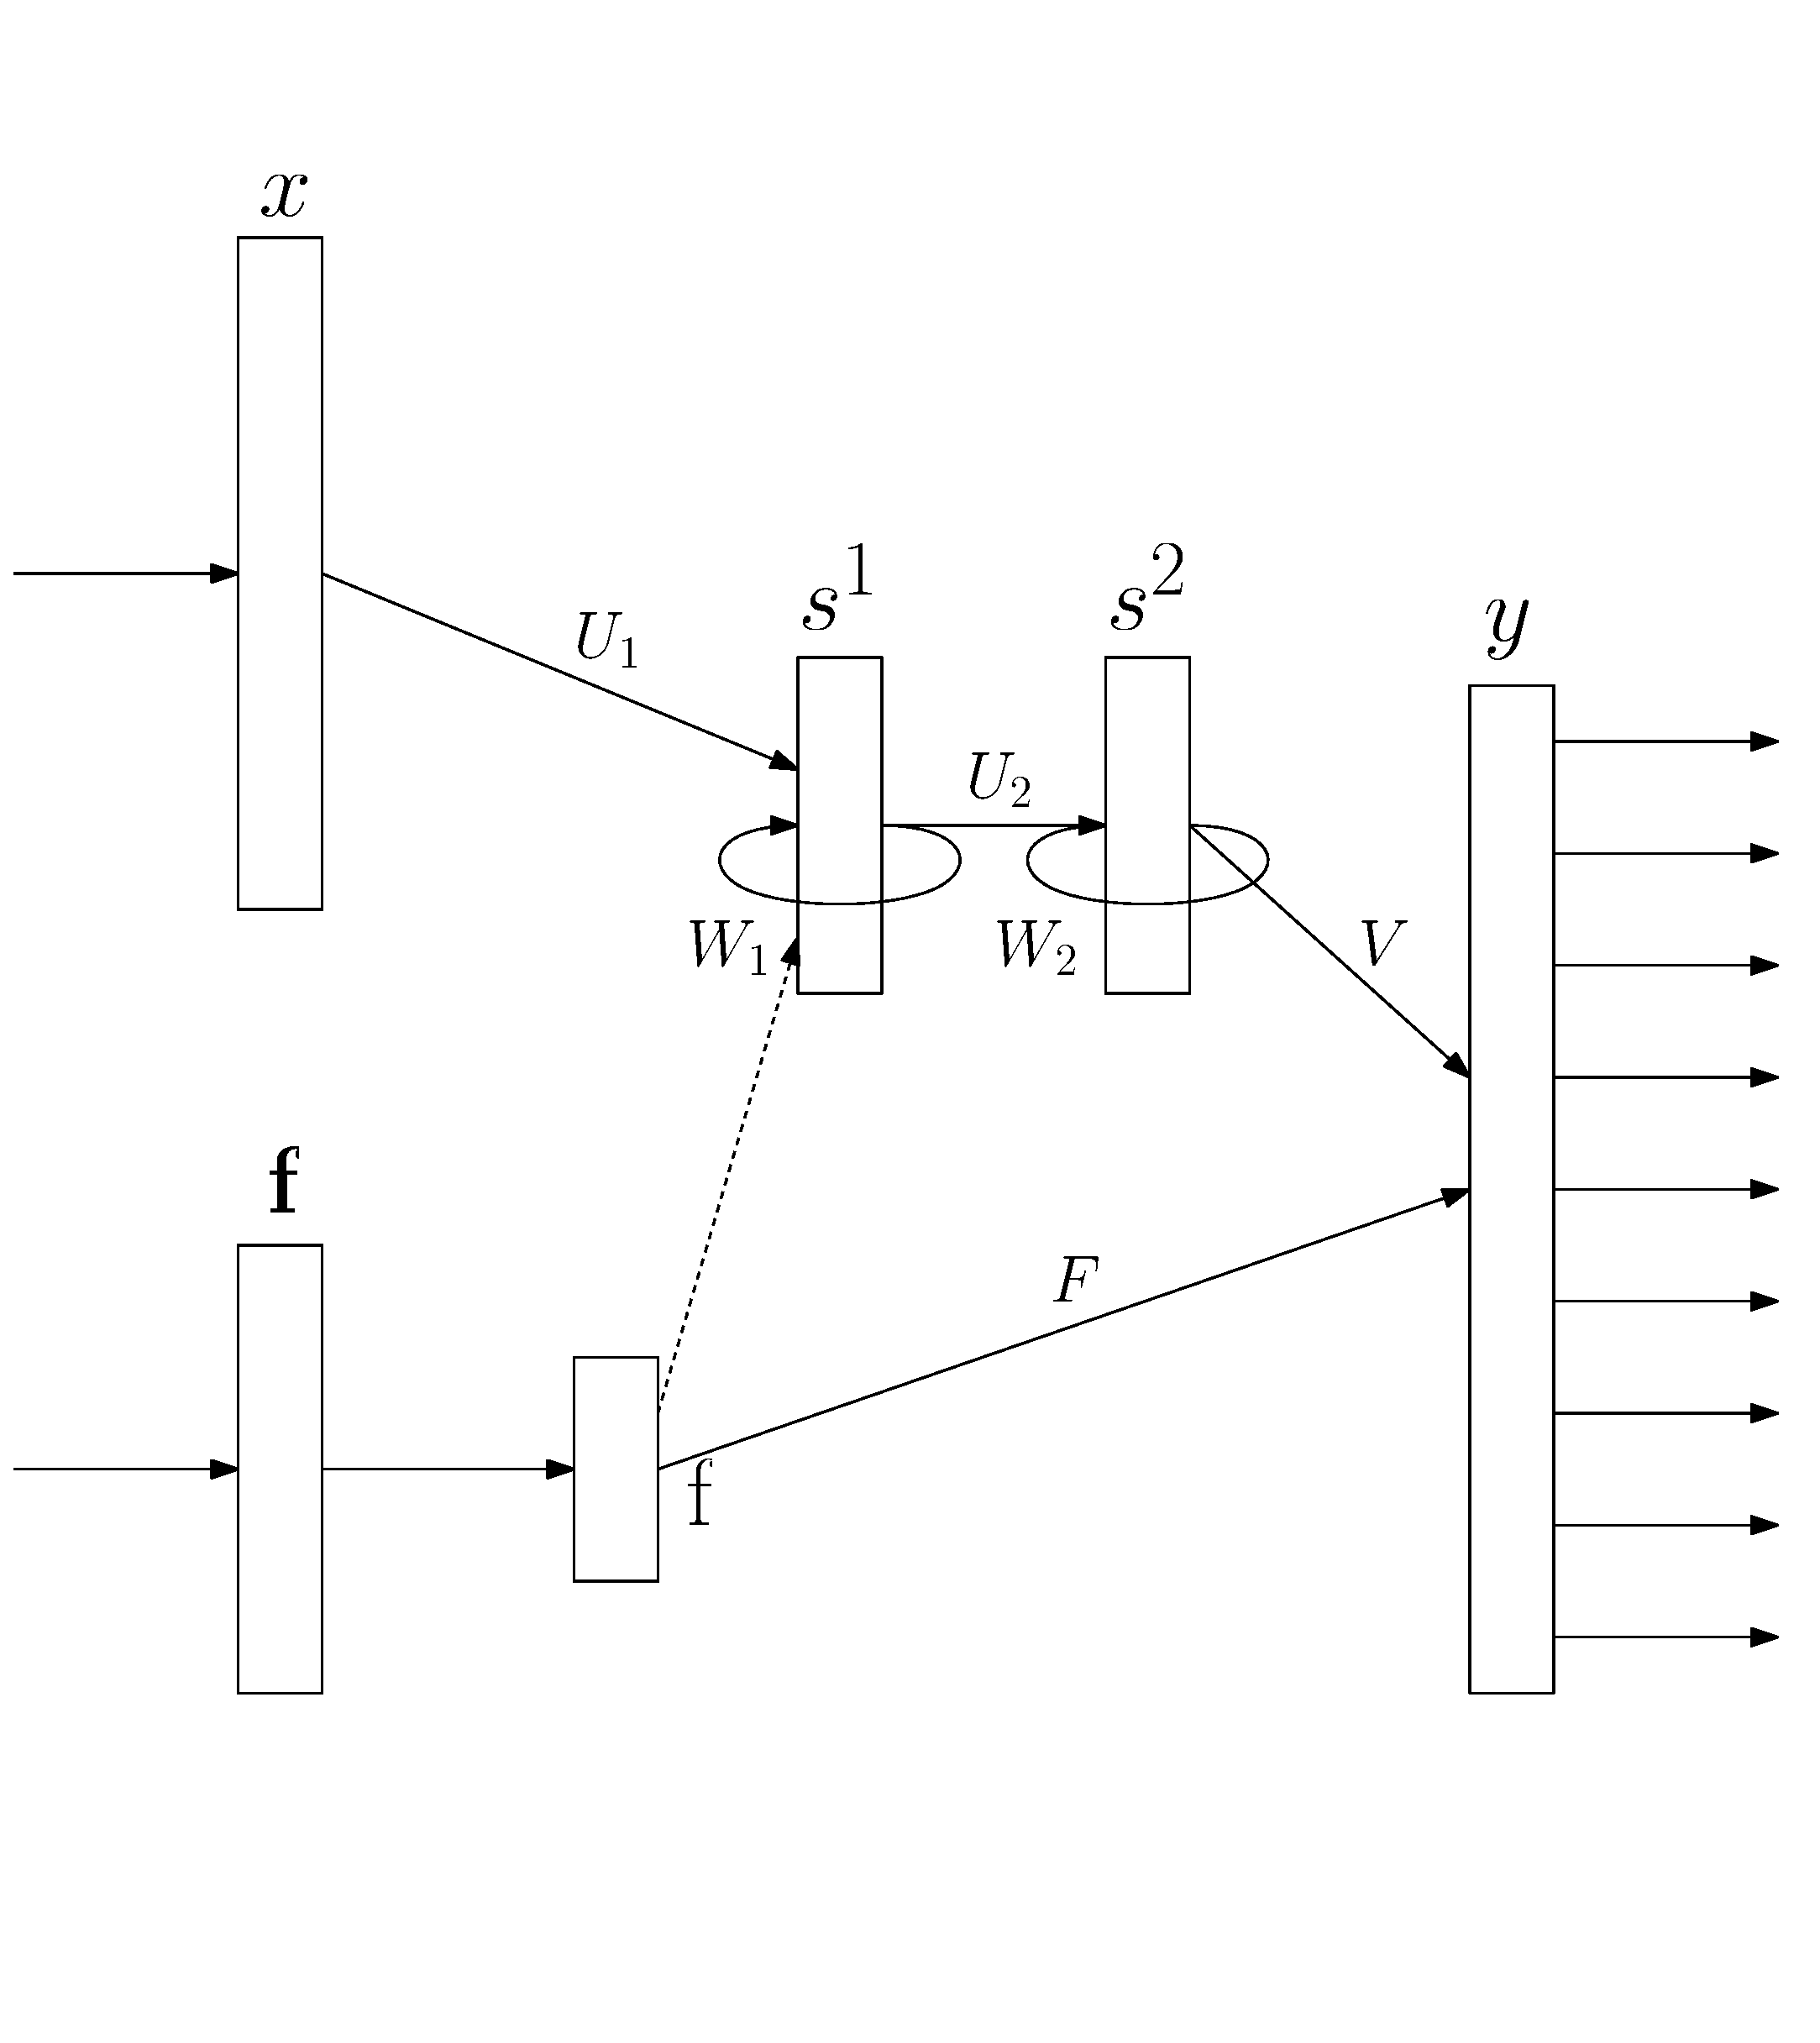
\includegraphics[width=\columnwidth]{ModelExtended2.pdf}
\caption{Extended recurrent language model with additional feature input $\textbf{f}$ and two LSTM-based hidden layers. The dashed line from the feature input to the first hidden layer represents an optional connection}
\label{fig:model-extended}
\end{figure}


\section{Experiments}
We evaluated both the factored language model and the extended language model on English-Chinese and English-Romanian language pairs. For each language pair we created the $n$-best list using our phrase-based MT system and used the models as additional feature in rescoring.

\subsection{System Description}
The baseline system is an in-house implementation of the phrase-based approach and is used to generate $n$-best lists on all the available training data. The English-Chinese system is trained on the TED and UN corpus, optimized and rescored on the TED dev2010 and tested on the test2010 corpora.
The English-Romanian system is trained on the corpora of WMT 2015 Shared Translation Task, optimized on the first half of news-dev 2016 and tested on the second half of news-dev 2016. In addition, for rescoring a subset of 2000 sentences of the SETimes corpus is used for further optimization.
The English-Chinese baseline system uses two word-based language models, and 12 features in total to create an $n$-best list of size 3000.
The English-Romanian baseline system uses two word-based language models, 2 cluster-based models using 50, 1000 or 1000 clusters, and a POS-based language model. In total 22-23 features are used to generate an $n$-best list of size 300. A full system description can be found in \cite{niehuesusing}.
For decoding, both language pairs are optimized using minimum error rate training. The same is used for rescoring of English-Chinese, whereas English-Romanian used ListNet to rerank the $n$-best list.
All RNN-based language models for both language pairs are trained on the target side of the parallel training data. The English-Chinese system uses a vocabulary of 10K, while the English-Romanian system uses a vocabulary of 5K words. For word level side information word categories are extracted from Wikipedia as described in \ref{sec:word-level} as input into the factored language model.
For sentence level side information, as described in \ref{sec:sentence-level}, an additional web-crawled Chinese lexicon from zdic.net \footnote{\label{foot:zdic} http://www.zdic.net/} is used in the English-Chinese system to show the model's performance independently from a specific encyclopedia.


\subsection{English-Chinese}
In the first experiment of English-Chinese we used the scores of the factored language model in addition to the baseline features, which is shown in Table \ref{tb:zh-factored}. BLEU score improvements over the basic recurrent language model are displayed in brackets. When using both words and Wikipedia categories the model performs 0.66 BLEU score points better in testing than the basic recurrent model using only words as input. Combining this model with the scores of a factored model with words and POS as factors produces a further increase of 0.14 points, resulting in an overall improvement of 0.84 BLEU points over the basic recurrent model.

\begin{table}
\caption{English-Chinese Factored Language Models}
\centering
  \begin{tabular}{ lll }
  	\hline
  	Model                  & devdata       & testdata      \\ \hline\hline
  	Baseline               & 14.69         & 17.05         \\
  	+RNNLM                 & 14.7          & 17.02         \\
  	+Factored LM POS       & 14.77         & 16.97         \\ \hline
  	+Factored LM Cat       & 14.89 (+0.12) & 17.63 (+0.66) \\
  	+Factored LM Cat + POS & 14.75 (-0.02) & 17.81 (+0.84) \\ \hline
  \end{tabular}
  \label{tb:zh-factored}
\end{table}

In a second experiment, extended language models using different methods to compute the feature input vector are studied. Tfidf, LSA and LDA are used for similar document ranking as well as vector representation. It is worth mentioning that the method for ranking can be paired with a different choice for representation. The performance results of various combinations of pairings are presented in Table \ref{tb:zh-extended-diff-features}. Although all combinations result in better rescoring performance compared to the basic recurrent model, choosing the same method for both tasks mostly achieve a noticeable higher boost. For example, tfidf creates an increase of 0.63 points on the basic recurrent model, LSA an increase of 0.78. The only exception to this rule is LDA. One reason for this could be suboptimal parameter picks for this generally more complex generative model. Despite the slightly better performance of LSA, tfidf is employed in the following experiments due to its simplicity and, thus, faster training and evaluation.

\begin{table}
\caption{Extended Language Models: Overview of different feature vectors}
\centering
  \begin{tabular}{llll}
  	\hline
  	Rank     & Vect  & devdata       & testdata      \\ \hline\hline
  	Baseline &       & 14.70         & 17.02         \\ \hline
  	TFIDF    & TFIDF & 14.78 (+0.08) & 17.68 (+0.63) \\
  	LSA      & TFIDF & 14.78 (+0.08) & 17.31 (+0.29) \\
  	LSA      & LSA   & 14.83 (+0.13) & 17.80 (+0.78) \\
  	LDA      & TFIDF & 14.79 (+0.09) & 17.41 (+0.39) \\
  	LDA      & LDA   & 14.79 (+0.09) & 17.27 (+0.25)
  \end{tabular}
  \label{tb:zh-extended-diff-features}
\end{table}

In order to test the efficiency of this model independently from the characteristics of the  underlying encyclopedia  source, a Chinese lexicon is crawled from zdic.net \footnotemark[\ref{foot:zdic}]. It contrasts Wikipedia in the variety and length of definitions. The lexicon provides more but shorter compact explanations for all type of words, particularly verbs. Despite the difference in content, the use of the lexicon shows an increase of 0.56 BLEU points, similar to that of Wikipedia as shown in Table \ref{tb:zh-extended-diff-sources}.

\begin{table}
\caption{Extended Language Models: Comparison between different encyclopedia sources}
\centering
  \begin{tabular}{lll}
  	\hline
  	Model    & devdata       & testdata      \\ \hline\hline
  	Baseline & 14.69         & 17.05         \\
  	+RNNLM   & 14.7          & 17.02         \\ \hline
  	+Wiki    & 14.78 (+0.08) & 17.68 (+0.66) \\
  	+Dict    & 14.91 (+0.21) & 17.58 (+0.56) \\ \hline
  \end{tabular}
  \label{tb:zh-extended-diff-sources}
\end{table}

An overview of all the models and their perplexities is given in Table \ref{tb:PPL}. All models exhibit an evident reduction in perplexity compared to the basic recurrent model, which goes along with the previous rescoring results.

\begin{table} 
  \caption{Model Perplexities}
  \centering
  \begin{tabular}{ ll}
  	\hline
  	Model               & PPL    \\ \hline\hline
  	RNNLM               & 128.17 \\ \hline
  	Factored LM POS     & 110.86 \\
  	Factored LM Cat     & 109.73 \\
  	Factored LM Cat+POS & 110.38 \\ \hline
  	WIKI                & 120.60 \\
  	ZDICT               & 118.85 \\ \hline
  \end{tabular}
  \label{tb:PPL}
\end{table}


As indicated by Figure \ref{fig:model-extended}, an additional connection was established between the feature layer and the first hidden layer in another experiment. Using tfidf the model gained a small increase of +0.16 BLEU on the model with single connection and a total of +0.79 BLEU on the simple recurrent model, as shown in Table \ref{tb:zh-extended-both}.


\begin{table}
\caption{Extended Language Models: Connecting feature input with two layers}
\centering
  \begin{tabular}{lll}
  	\hline
  	Model               & devdata       & testdata      \\ \hline\hline
  	Baseline+RNNLM      & 14.70         & 17.02         \\ \hline
  	Baseline+TFIDF      & 14.78 (+0.08) & 17.68 (+0.63) \\
  	Baseline+2Con TFIDF & 14.74 (+0.04) & 17.81 (+0.79)
  \end{tabular}
  \label{tb:zh-extended-both}
\end{table}


\subsection{English-Romanian}
In the previous work \anony{\cite{niehuesusing}} , the factored language model for English-Romanian integrated four factors: the word's surface form, POS, and word clusters with 100 and 1000 class respectively. Our experiment builds on top of \cite{niehuesusing}, which used for all systems a vocabulary of 5K, and the same denotations are used to illustrate the following results. In the first experiment, only the factored language models are evaluated without the baseline system. The system from the previous work with all four factors as input and prediction reached a BLEU score of 28.54, as shown in Table \ref{tb:ro-factored-single}. This model will serve as reference for our models. After adding our extracted Wikipedia word categories to the factors, we achieved improvement of 0.17 and 0.30 BLEU points respectively.


\begin{table}
\caption{Factored Language Models: Single Scores}
\centering
  \begin{tabular}{lll}
  	\hline
  	Input            & Prediction   & Single        \\ \hline\hline
  	Word             & Word         & 27.88         \\
  	All factors      & All factors  & 28.54         \\ \hline
  	+Cat (Nouns)     & +Cat (Nouns) & 28.71 (+0.17) \\
  	+Cat (All Words) & +Cat (All)   & 28.84 (+0.30)
  \end{tabular}
  \label{tb:ro-factored-single}
\end{table}

Table \ref{tb:ro-factored-combi} shows the results of model features used in addition to the baseline system in three configurations, which are evaluated using just the joint probability. 
Adding word tags for all word types achieved an improvement of about 0.1 BLEU points in two configurations over the reference model.

\begin{table}
\caption{Factored Language Models: End Scores}
\centering
  \begin{tabular}{llll}
  	\hline
  	Model                    & Conf1   & Conf2   & Conf3   \\ \hline\hline
  	Baseline                 & 29.86   & 30.00   & 29.75   \\
  	+All factors             & 29.94   & 30.01   & 30.01   \\ \hline
  	+All factors + Nouns     & 29.94   & 30.31   & 29.99   \\
  	                         & (+0.00) & (+0.30) & (-0.02) \\
  	+All factors + All Words & 29.95   & 30.13   & 30.14   \\
  	                         & (+0.01) & (+0.12) & (+0.13)
  \end{tabular}
  \label{tb:ro-factored-combi}
\end{table}


\section{Conclusion}
In this work, we proposed two approaches to integrate higher level information from encyclopediatic sources into neural network language models. The first takes advantage of Wikipedia, which is one of the fastest growing encyclopedias. The second approach takes a continuous space vectors as additional input which enables incorporation of more complex side information on the sentence level. In addition, we  also introduce three different methods how to prepare the additional data and represent it in the correct form.
By using of more complex information from large independent sources, we have improved the translation system on two different language pairs.  
This work plays a key role for low-ressource languages, that often lack sufficient training data. 



\section{Acknowledgements}
%This work was funded by the CLICS Exchange Program.

\begin{comment}

The IWSLT 2015 organizing committee would like to thank the
organizing committees of INTERSPEECH 2004 for their
help and for kindly providing the template files.

\begin{itemize}
%\itemsep -1.3mm
\item Proceedings will be printed in A4 format. The layout is designed 
so that files, when printed in US Letter format, include all material 
but margins are not symmetric. 
Although this is not an absolute requirement, if at all possible,
{\bf PLEASE TRY TO MAKE YOUR SUBMISSION IN A4 FORMAT.}
\item Two columns are used except for the title part and possibly for large 
figures that need a full page width.
\item Left margin is 20 mm.
\item Column width is 80 mm.
\item Spacing between columns is 10 mm.
\item Top margin 25 mm (except first page 30 mm to title top).
\item Text height (without headers and footers) is maximum 235 mm.
\item Headers and footers must be left empty (they will be added for 
printing).
\item Check indentations and spacings by comparing to this 
example file (in pdf format).
\end{itemize}



\subsubsection{Headings}

Section headings are centered in boldface
with the first word capitalized and the rest of the heading in 
lower case. Sub-headings appear like major headings, except they 
start at the left margin in the column.
Sub-sub-headings appear like sub-headings, except they are in italics 
and not boldface. See the examples given in this 
file. No more than 3 levels of headings should be used.

\subsection{Text font}

Times or Times Roman font is used for the main text. Recommended 
font size is 9 points which is also the minimum allowed size.
Other font types may be used if needed for 
special purposes. While making the final PostScript file, 
remember to include all fonts!

\LaTeX\ users: DO NOT USE Computer Modern FONT FOR TEXT (Times is 
specified in the style file). If possible, make the final 
document using POSTSCRIPT FONTS.
This is necessary given that, for example, equations with 
non-ps Computer Modern are very hard to read on screen.

\subsection{Figures}

All figures must be centered on the column (or page, if the figure spans 
both columns).
Figure captions should follow each figure and have the format given in 
Fig.~\ref{spprod}.

Figures should preferably be line drawings. If they contain gray 
levels or colors, they should be checked to print well on a 
high-quality non-color laser printer.

\subsection{Tables}

An example of a table is shown as Table \ref{table1}. Somewhat 
different styles are allowed according to the type and purpose of the 
table. The caption text may be above or below the table.

\begin{table}
\caption{\label{table1} {\it This is an example of a table.}}
\vspace{2mm}
\centerline{
\begin{tabular}{|c|c|}
\hline
ratio & decibels \\
\hline  \hline
1/1 & 0 \\
2/1 & $\approx 6$ \\
3.16 & 10 \\
10/1 & 20 \\ 
1/10 & -20 \\
\hline
\end{tabular}}
\end{table}

\subsection{Equations}

Equations should be placed on separate lines and numbered. Examples 
of equations are given below.
Particularly,
%
%\vspace{-3mm}
\begin{equation}
x(t) = s(f_\omega(t))
\label{eq1}
\end{equation}
where \(f_\omega(t)\) is a special warping function
\begin{equation}
f_\omega(t)=\frac{1}{2\pi j}\oint_C \frac{\nu^{-1k}d\nu}
{(1-\beta\nu^{-1})(\nu^{-1}-\beta)}
\label{eq2}
\end{equation}
A residue theorem states that
\begin{equation}
\oint_C F(z)dz=2 \pi j \sum_k Res[F(z),p_k]
\label{eq3}
\end{equation}
Applying (\ref{eq3}) to (\ref{eq1}), 
it is straightforward to see that
\begin{equation}
1 + 1 = \pi
\label{eq4}
\end{equation}

Make sure to use \verb!\eqref! when refering to equation numbers.
Finally we have proven the secret theorem of all speech sciences (see
equation~\eqref{eq3} above).  No more math is needed to show how 
useful the result is! 

\begin{figure}[t]
\centerline{\epsfig{figure=figure,width=40mm}}
\caption{{\it Schematic diagram of speech production.}}  
\label{spprod}
\end{figure}

\subsection{Hyperlinks}

Hyperlinks can be included in your paper. Moreover, be aware that the paper
submission procedure includes the option of specifying a hyperlink for
additional information.  This hyperlink will be included in the CD-ROM.
Particularly pay attention to the possibility, from this single hyperlink, to
have further links to information such as other related documents, sound or
multimedia.

If you choose to use active hyperlinks in your paper, 
please make sure that they present no problems in printing to paper. 

\subsection{Page numbering}

Final page numbers will be added later to the document
electronically. 
{\em Please don't make any headers or footers!}.

\subsection{References}

The reference format is the standard for IEEE publications.
References should be numbered in order of appearance, 
for example \cite{ES1}, \cite{ES2}, and \cite{ES3}. 

\section{Experiments}
Please make sure to give all the necessary details regarding your experimental 
setting so as to ensure that your results could be reproduced by other teams. 

\section{Conclusions}

This paper has described a novel approach for doing wonderful stuff such as ...
content...
\end{comment}

%
\bibliographystyle{IEEEtran}
\bibliography{references}
%\begin{comment}
%\bibitem[1]{ES1} Smith, J. O. and Abel, J. S., 
%``Bark and {ERB} Bilinear Transforms'', 
%IEEE Trans. Speech and Audio Proc., 7(6):697--708, 1999.  
%\bibitem[2]{ES2} Lee, K.-F., Automatic Speech Recognition: 
%The Development of the 
%SPHINX SYSTEM, Kluwer Academic Publishers, Boston, 1989.
%\bibitem[3]{ES3} Rudnicky, A. I., Polifroni, Thayer, E. H.,
% and Brennan, R. A.  
%"Interactive problem solving with speech", J. Acoust. Soc. Amer., 
%Vol. 84, 1988, p S213(A).
%\end{comment}
\end{document}

